% \subsection{Digital Humanities}
%
% Anne Burdick, Johanna Drucker, Peter Lunefeld, Todd Presner and Jeffrey Schnapp (referred to as "the authors" in this section) have collaboratively written an authoritative manifesto for the field of digital humanities (DH) (\citep{Burdick2012}. Computing has had a big impact on the humanities as a discipline so much so that DH was born of the encounter between the two \citep[p.3]{Burdick2012}. In essence, it is characterised by \textbf{collaboration, transdisciplinarity and an engagement with computing} \citep[p.122]{Burdick2012} but it should not simply be reduced to doing the humanities digitally \citep[p.101]{Burdick2012}. It spans across many traditional areas of research, such as literature, philosophy, history, art, music, design and of course computer science.
%
% \begin{draft}
% Transliteracy\footnote{Sue Thomas et al. define transliteracy as "the ability to read, write and interact across a range of platforms, tools and media from signing and orality through handwriting, print, TV, radio and film, to digital social networks." \citep{Thomas2007}} therefore is fundamental \citep{Thomas2007};
% \end{draft}
%
% "The field of Digital Humanities may see the emergence of polymaths who can 'do it all'": who can research, write, shoot, edit, code, model, design, network, and dialogue with users. \citep[p.15]{Burdick2012} DH encompasses several core activities which on various levels depend on and support each other.
%
% \begin{description}
% \item [Design]:	Shape, scheme, inform, experience, position, narrate,
% 					interpret, remap/reframe, reveal, deconstruct, reconstruct,
% 					situate, critique
% \item [Curation, analysis, editing, modelling]:	Digitise, classify, describe, metadata, organise, navigate
% \item [Computation, processing]: Disambiguate, encode, structure, procedure, index, automate, sort, search, calculate, match
% \item [Networks, infrastructure]:	Cultural, institutional, technical, compatible, interoperable, flexible, mutable, extensible
% \item [Versioning, prototyping, failures]:	Iterate, experiment, take-risks, redefine, beta-test
% \end{description}
%
% \begin{draft}
% IF THE STUDY OF ART OR HUMAN CREATIVITY FALLS WITHIN HUMANITIES RESEARCH, THEN COMP CREAT SHOULD FALL WITHIN DIGITAL HUMANITIES, RIGHT, AND USE THE TOOLS AND METHODS AVALIBALE.
% \end{draft}
%
% \subsubsection{DESIGN}
% The authors suggest that "for digital humanists, design is a creative practice harnessing cultural, social, economic, and technological constraints in order to bring systems and objects into the world." \citep[p.13]{Burdick2012}
%
% In generative mode, these designers shape structural logics, rhetorical schemata, information hierarchies, experiential qualities, cultural positioning, and narrative strategies. When working analytically, their task is to visually interpret, remap or reframe, reveal patterns, deconstruct, reconstruct, situate, and critique. \citep[p.12]{Burdick2012}
%
% \subsubsection{CURATION, ANALYSIS, EDITING, MODELING}
% \begin{quote}
% "digital activity: digitization, classification, description and metadata, organization, and navigation." \citep[p.17]{Burdick2012}
% \end{quote}
%
% \begin{quote}
% "Involving archives, collections, repositories, and other aggregations of materials, CURATION is the selection and organization of materials in an interpretive framework, argument, or exhibit." \citep[p.17]{Burdick2012}
% \end{quote}
%
% \begin{quote}
% "The parsing of the cultural record in terms of questions of authenticity, origin, transmission, or production is one of the foundation stones of humanistic scholar- ship upon which all other interpretive work depends. But editing is also productive and generative, and it is the suite of rhetorical devices that make a work. Editing is the creative, imaginative activity of making, and as such, design can be also seen as a kind of editing" \citep[p.18]{Burdick2012}
% \end{quote}
%
% \begin{quote}
% "MODELING highlights the notion of content models—shapes of argument expressed in information structures and their design". \citep[p.18]{Burdick2012}
% \end{quote}
%
% \subsubsection{COMPUTATION, PROCESSING}
% \begin{quote}
% "interpretation is rethought through the encounter with computational methods and [] computational methods are rethought through the encounter with humanistic modes of knowing." \citep[p.103]{Burdick2012}
% \end{quote}
%
% \begin{quote}
% "Humanists have begun to use programming languages. But they have yet to create programming languages of their own: languages that can come to grips with, for example, such fundamental attributes of cultural communication and traditional objects of humanistic scrutiny as nuance, inflection, undertone, irony, and ambivalence." \citep[p.103]{Burdick2012}
% \end{quote}
%
% \begin{figure}[htbp]
%   \centering
%     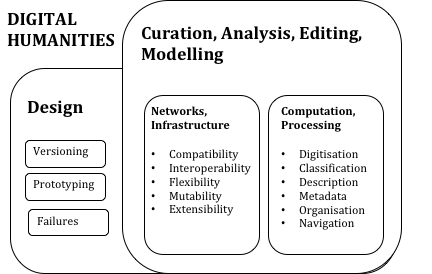
\includegraphics{images/dh.png}
%   \caption[Digital Humanities]{Digital Humanities model}
%   \label{fig:Digital_Humanities}
% \end{figure}
%
% \subsubsection{NETWORKS, INFRASTRUCTURE}
% \begin{quote}
% "Designing and building digital projects depend on knowledge of these fundamentals and on a nuanced understanding of the net- worked environments in which the projects will develop and variously reside." \citep[p.17]{Burdick2012}
% \end{quote}
%
% \begin{quote}
% "Digital work takes place in the real world, and humanists once accus- tomed to isolated or individualized modes of production must now grapple with complex partnerships and with insuring the long-term availability and viability of their scholarship" \citep[p.21]{Burdick2012}
% \end{quote}
%
% \subsubsection{VERSIONING, PROTOTYPING, FAILURES}
% \begin{quote}
% "one of the strongest attributes of the field is that the iterative versioning of digital projects fosters experimentation, risk-taking, redefinition, and sometime failure." \citep[p.21]{Burdick2012}
% \end{quote}
%
% \begin{draft}
% SOUNDS LIKE SOFTWARE ENGINEERING
% \end{draft}
%
% \begin{quote}
% "It is important that we do not short-circuit this experimental process in the rush to normalize practices, standardize methodologies, and define evaluative metrics." \citep[p.21]{Burdick2012}
% \end{quote}
%
% \begin{draft}
% argument for creative computing too
% \end{draft}
%
% \subsubsection{Field map of digital humanities: emerging methods and genres}\citep[p.29-60]{Burdick2012}
%
% \begin{verbatim}
% •	enhanced critical curation
% o	digital collections
% o	multimedia critical editions
% o	object-based argumentation
% o	expanded publication
% o	experiential and spatial
% o	mixed physical and digital
% •	augmented editions and fluid textuality
% o	structured mark-up
% o	natural language processing
% o	relational rhetoric
% o	textual analysis
% o	variants and versions
% o	mutability
% •	scale: the law of large numbers
% o	quantitative analysis
% o	text-mining
% o	machine reading
% o	digital cultural record
% o	algorithmic analysis
% •	distant/close, macro/micro, surface/depth
% o	large-scale patterns
% o	fine-grained analysis
% o	close reading
% o	distant reading
% o	differential geographies
% •	cultural analytics, aggregation, and data-mining
% o	parametrics
% o	cultural mash-ups
% o	computational processing
% o	composite analysis
% o	algorithm design
% •	visualization and data design
% o	data visualization
% o	mapping
% o	information design
% o	simulation environments
% o	spatial argument
% o	modelling knowledge
% o	visual interpretation
% •	locative investigation and thick mapping
% o	spatial humanities
% o	digital cultural mapping
% o	interconnected sites
% o	experimental navigation
% o	geographic information systems (GIS)
% o	stacked data
% •	the animated archive
% o	user communities
% o	permeable walls
% o	active engagement
% o	bottom-up curation
% o	multiplied access
% o	participatory content creation
% •	distributed knowledge production and performative access
% o	global networks
% o	ambient data
% o	collaborative authorship
% o	interdisciplinary teams
% o	use as performance
% o	crowd-sourcing
% •	humanities gaming
% o	user engagement
% o	rule-based play
% o	rich interaction
% o	virtual learning environments
% o	immersion and simulation
% o	narrative complexity
% •	code, software, and platform studies
% o	narrative structures
% o	code as text
% o	computational processes
% o	software in a cultural context
% o	encoding practices
% •	database documentaries
% o	variable experience
% o	user-activated
% o	multimedia prose
% o	modular and combinatoric
% o	multilinear
% •	repurposable content and remix culture
% o	participatory Web
% o	read/write/rewrite
% o	platform migration
% o	sampling and collage
% o	meta-medium
% o	inter-textuality
% •	pervasive infrastructure
% o	extensible frameworks
% o	heterogeneous data streams
% o	polymorphous browsing
% o	cloud computing
% •	ubiquitous scholarship
% o	augmented reality
% o	web of things
% o	pervasive surveillance and tracking
% o	ubiquitous computing
% o	deterritorialization of humanistic practice
% \end{verbatim}
%
% \begin{draft}
% quantifiable and repeatable phenomena versus complex dynamics of interpretation, cultural meanings, probabilistic modelling, interpretive mapping, subjective visualizations, and self-customizing navigation \citep[p.103]{Burdick2012}
% \end{draft}
%
% \subsubsection{TOOLS}
% \begin{quote}
% "Building tools around core humanities concepts: subjectivity, ambiguity, contingency, observer-dependent variables in the production of knowledge: holds the promise of expanding current models of knowledge. As such, the next generation of digital experimenters could contribute to humanities theory by forging tools that quite literally embody humanities centred views regarding the world." \citep[p.104]{Burdick2012}
% \end{quote}
%
% \begin{quote}
% "Tools are not just tools. They are cognitive interfaces that presuppose forms of mental and physical discipline and organization. By scripting an action, they produce and transmit knowledge, and, in turn, model a world." \citep[p.105]{Burdick2012}
% \end{quote}
%
% \begin{quote}
% "For all its potential interest, a humanities-centered computational environment could well end up distancing humanistic work from the mainstream of digital society, either because of its specialized or speculative character, or because the values that inform its architecture are at odds with the needs of business for standardization, quantitative metrics, and disambiguation." \citep[p.105]{Burdick2012}
% \end{quote}
%
% \begin{shaded}
% Summary\\
% •	Collaborative, Transdisciplinary and Computing
% \end{shaded}
%
% \subsection{Computer Ethics}
%
% \begin{draft}
% ETHICS: PROCESS< PRODUCT< PURPOSE\\
% ROBOT ETHICS: similar to 4-p’s of creativity \citep{McBride2013}\\
%
% it has three actors: Robot engineer, client and user.
%
% 4 approaches:\\
% •	challenge the myth of autonomy\\
% •	Developing practice-based approaches (in context of it purpose and environment)\\
% •	Managing ethical variety\\
% •	A model for human0centred robot ethics\\
%
% Virtuous robot:\\
% •	Human-centred\\
% •	Man-machine interdependency\\
% •	Practice based (context)\\
% •	Ethical variety
% \end{draft}
%
% \subsection{Similarities and Differences}
%
% We had previously differentiated between creative computing and computational creativity:
%
% \begin{quote}
% "Intuitively the former is about doing computations in a creative way, while the latter is about achieving creativity through computation. You can think of the latter falling into the artificial intelligence category (using formal computational methods to mimic creativity as a human trait, see also [18]) and the former being a more poetic endeavour of how the computing itself is done, no matter what the actual purpose of the program is." \citep{Hugill2013}
% \end{quote}
%
% The differences are subtle but clear.
%
% \begin{table}[htbp]
% \centering
% \begin{tabular}{|l|p{5cm}|l|}
% \hline
% \textbf{Creative Computing} & \textbf{Digital Humanities} & \textbf{Computational Creativity} \\ \hline
% Motivation  & Design & Intentionality \\ \hline
% Ideation & Curation, Analysis, Editing, Modeling and Networks, Infrastructure & Framing \\ \hline
% Implementation & Computation, Processing & Process \\ \hline
% Operation & Versioning, Prototyping, Failures & Product \\ \hline
% \end{tabular}
% \caption[Creative Computing vs Digital Humanities vs Computational Creativity]{Comparison of Creative Computing vs Digital Humanities vs Computational Creativity}
% \end{table}
%
% \begin{table}[htbp]
% \centering
% \begin{tabular}{|l|l|l|}
% \hline
% \textbf{4 step model} & \textbf{4 P Model} & \textbf{Problem Solving} \\ \hline
% Preparation   & Person         & Understand  \\ \hline
% Incubation    & Press/Context  & Plan        \\ \hline
% Illumination  & Process        & Carry Out   \\ \hline
% Verification  & Product        & Look back   \\ \hline
% \end{tabular}
% \caption[4 Step Model vs 4 P Model vs Problem Solving]{Comparison of 4 Step Model vs 4 P Model vs Problem Solving}
% \end{table}
%
% \begin{comment}
% How does ethics fit into this?
% \end{comment}
